% This file was created with matplot2tikz v0.4.0.
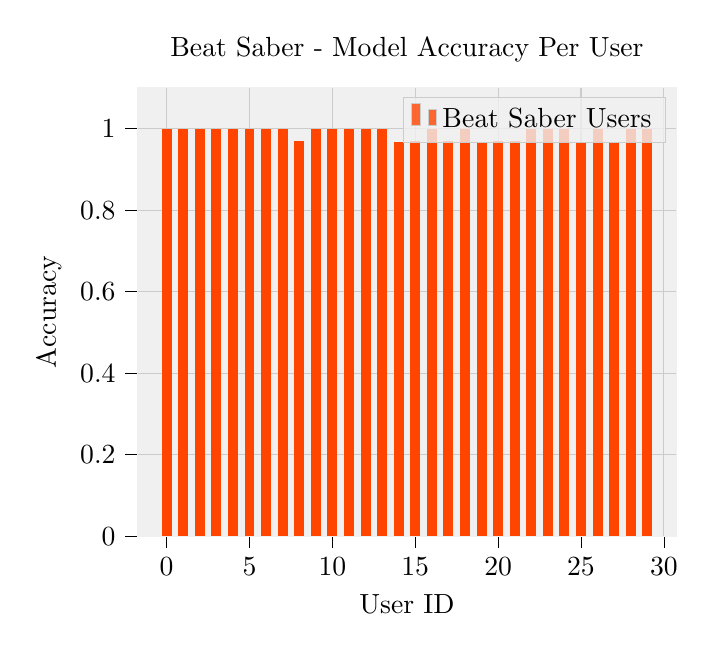
\begin{tikzpicture}

\definecolor{lightgray203}{RGB}{203,203,203}
\definecolor{lightgray204}{RGB}{204,204,204}
\definecolor{orangered}{RGB}{255,69,0}
\definecolor{whitesmoke240}{RGB}{240,240,240}

\begin{axis}[
axis background/.style={fill=whitesmoke240},
axis line style={whitesmoke240},
legend cell align={left},
legend style={fill opacity=0.8, draw opacity=1, text opacity=1, draw=lightgray204, fill=whitesmoke240},
tick align=outside,
tick pos=left,
title={Beat Saber - Model Accuracy Per User},
x grid style={lightgray203},
xlabel={User ID},
xmajorgrids,
xmin=-1.78, xmax=30.78,
xtick style={color=black},
y grid style={lightgray203},
ylabel={Accuracy},
ymajorgrids,
ymin=0, ymax=1.1,
ytick style={color=black}
]
\draw[draw=none,fill=orangered,very thin] (axis cs:-0.3,0) rectangle (axis cs:0.3,1);
\addlegendimage{ybar,ybar legend,draw=none,fill=orangered,very thin}
\addlegendentry{Beat Saber Users}

\draw[draw=none,fill=orangered,very thin] (axis cs:0.7,0) rectangle (axis cs:1.3,1);
\draw[draw=none,fill=orangered,very thin] (axis cs:1.7,0) rectangle (axis cs:2.3,1);
\draw[draw=none,fill=orangered,very thin] (axis cs:2.7,0) rectangle (axis cs:3.3,1);
\draw[draw=none,fill=orangered,very thin] (axis cs:3.7,0) rectangle (axis cs:4.3,1);
\draw[draw=none,fill=orangered,very thin] (axis cs:4.7,0) rectangle (axis cs:5.3,1);
\draw[draw=none,fill=orangered,very thin] (axis cs:5.7,0) rectangle (axis cs:6.3,1);
\draw[draw=none,fill=orangered,very thin] (axis cs:6.7,0) rectangle (axis cs:7.3,1);
\draw[draw=none,fill=orangered,very thin] (axis cs:7.7,0) rectangle (axis cs:8.3,0.96969696969697);
\draw[draw=none,fill=orangered,very thin] (axis cs:8.7,0) rectangle (axis cs:9.3,1);
\draw[draw=none,fill=orangered,very thin] (axis cs:9.7,0) rectangle (axis cs:10.3,1);
\draw[draw=none,fill=orangered,very thin] (axis cs:10.7,0) rectangle (axis cs:11.3,1);
\draw[draw=none,fill=orangered,very thin] (axis cs:11.7,0) rectangle (axis cs:12.3,1);
\draw[draw=none,fill=orangered,very thin] (axis cs:12.7,0) rectangle (axis cs:13.3,1);
\draw[draw=none,fill=orangered,very thin] (axis cs:13.7,0) rectangle (axis cs:14.3,0.967741935483871);
\draw[draw=none,fill=orangered,very thin] (axis cs:14.7,0) rectangle (axis cs:15.3,0.96875);
\draw[draw=none,fill=orangered,very thin] (axis cs:15.7,0) rectangle (axis cs:16.3,1);
\draw[draw=none,fill=orangered,very thin] (axis cs:16.7,0) rectangle (axis cs:17.3,0.96969696969697);
\draw[draw=none,fill=orangered,very thin] (axis cs:17.7,0) rectangle (axis cs:18.3,1);
\draw[draw=none,fill=orangered,very thin] (axis cs:18.7,0) rectangle (axis cs:19.3,0.96551724137931);
\draw[draw=none,fill=orangered,very thin] (axis cs:19.7,0) rectangle (axis cs:20.3,0.96969696969697);
\draw[draw=none,fill=orangered,very thin] (axis cs:20.7,0) rectangle (axis cs:21.3,0.96969696969697);
\draw[draw=none,fill=orangered,very thin] (axis cs:21.7,0) rectangle (axis cs:22.3,1);
\draw[draw=none,fill=orangered,very thin] (axis cs:22.7,0) rectangle (axis cs:23.3,1);
\draw[draw=none,fill=orangered,very thin] (axis cs:23.7,0) rectangle (axis cs:24.3,1);
\draw[draw=none,fill=orangered,very thin] (axis cs:24.7,0) rectangle (axis cs:25.3,0.96551724137931);
\draw[draw=none,fill=orangered,very thin] (axis cs:25.7,0) rectangle (axis cs:26.3,1);
\draw[draw=none,fill=orangered,very thin] (axis cs:26.7,0) rectangle (axis cs:27.3,0.96551724137931);
\draw[draw=none,fill=orangered,very thin] (axis cs:27.7,0) rectangle (axis cs:28.3,1);
\draw[draw=none,fill=orangered,very thin] (axis cs:28.7,0) rectangle (axis cs:29.3,1);
\end{axis}

\end{tikzpicture}
